\section{Project Model}



An example is the traditional waterfall model.
\\\\
The waterfall model is based on having detailed knowledge and understanding of the system and the requirements up front, and expects minimal errors and change executing each phase of the project.
\\\\
\begin{figure}
 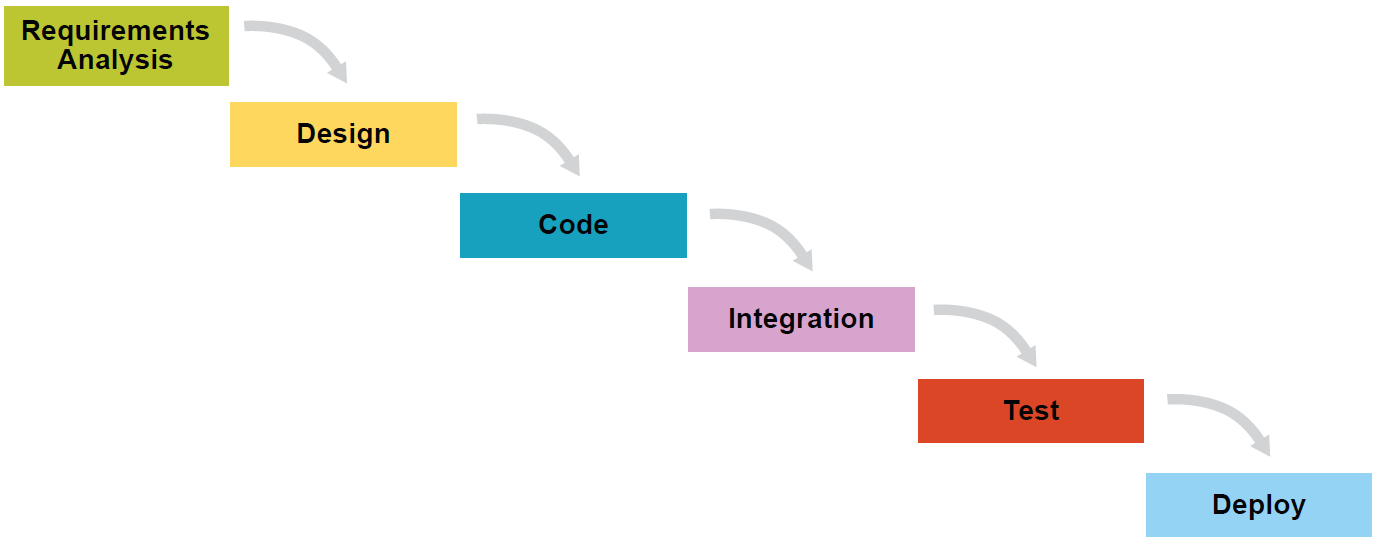
\includegraphics{VAPIQ-PICTURES/WaterFall.PNG}
 \caption{Fig 1: Waterfall Model}
\end{figure}


This model has its drawbacks. This is due to the fact that the model implies that the development team gets everything right from the start, and in reality this will most likely not be the case. Once a feature is ready

and therefore increases the risk of the system not meeting the stakeholders needs because they are brought in too late in the process.




%Once an application is in the testing stage, it is very difficult to go back and change something that was not well-thought out in the concept stage.
%No working software is produced until late during the life cycle.
%High amounts of risk and uncertainty.
%Not a good model for complex and object-oriented projects.
%Poor model for long and ongoing projects.
%Not suitable for the projects where requirements are at a moderate to high risk of changing.



%The systems engineering process must begin by discovering the real problems that need to be resolved, and identify the most probable or highest impact failures that can occur – systems engineering involves finding elegant solutions to these problems.

%Ken Schwaber co-developed the Scrum process with Jeff Sutherland in the early 1990s to help organizations struggling with complex development projects

